
前面的章节中已经使用了find\_package(),用来简化了整个过程。为了使项目可以通过这个指令访问,需要完成几个步骤,以便CMake可以将项目作为一个包来处理:

\begin{itemize}
\item 
目标可以重新定位。

\item 
将目标导出文件安装到标准位置。

\item 
为包创建配置文件和版本文件。
\end{itemize}

为什么目标需要重新定位,如何做到呢?

\subsubsubsection{11.4.1\hspace{0.2cm}理解可重定位目标}

安装解决了许多问题,但也引入了一些复杂性:CMAKE\_INSTALL\_PREFIX不仅是特定于平台的,而且还可以由用户在安装阶段使用-{}-prefix设置。然而,目标导出文件是在安装之前生成的,在构建阶段并不知道安装的工件将去哪里。看看下面的代码:

\begin{lstlisting}[style=styleCMake]
# chapter-11/01-export/src/CMakeLists.txt

add_library(calc STATIC calc.cpp)
target_include_directories(calc INTERFACE include)
\end{lstlisting}

本例中,将include目录添加到calc的include目录中。由于这是一个相对路径,CMake导出的目标生成将在此路径前加上CMAKE\_CURRENT\_SOURCE\_DIR的内容,该变量指向该列表文件所在的目录。

然而,这并不能解决问题。安装项目不再需要来自源文件或构建树的文件,所有内容(包括库头文件)都可复制到共享位置,例如Linux上的/usr/lib/calc/。我们不能在另一个项目中使用此代码段中定义的目标,因为目标的include目录路径仍然指向其源树。

CMake用两个生成器表达式解决了这个问题,将根据上下文过滤掉表达式:

\begin{itemize}
\item 
\$<BUILD\_INTERFACE>: 这包括常规构建的内容,但不包括安装内容。

\item 
\$<INSTALL\_INTERFACE>: 包括用于安装的内容,但不包括常规构建的内容。
\end{itemize}

下面的代码展示了如何在实践中使用:

\begin{lstlisting}[style=styleCMake]
# chapter-11/06-install-export/src/CMakeLists.txt

add_library(calc STATIC calc.cpp)
target_include_directories(calc INTERFACE
	"$<BUILD_INTERFACE:${CMAKE_CURRENT_SOURCE_DIR}/include>"
	"$<INSTALL_INTERFACE:${CMAKE_INSTALL_INCLUDEDIR}>"
)
set_target_properties(calc PROPERTIES
	PUBLIC_HEADER src/include/calc/calc.h
)
\end{lstlisting}

对于常规的构建,calc目标属性INTERFACE\_INCLUDE\_DIRECTORIES的值将展开:

\begin{tcblisting}{commandshell={}}
"/root/examples/chapter-11/05-package/src/include" ""
\end{tcblisting}

空双引号表明排除INSTALL\_INTERFACE中的值,计算为空字符串。安装时,值会像这样展开:

\begin{tcblisting}{commandshell={}}
"" "/usr/lib/calc/include"
\end{tcblisting}

这一次,BUILD\_INTERFACE生成器表达式中提供的值计算为空字符串,所以只剩下来自另一个生成器表达式的值。

关于CMAKE\_INSTALL\_PREFIX还有一句话:这个变量不应该用作目标中指定路径的组件。其将在构建阶段进行计算,使路径成为绝对路径,不一定与安装阶段提供的路径相同(用户可以使用-{}-prefix选项)。相反,使用\$<install\_prefix>生成器表达式:

\begin{lstlisting}[style=styleCMake]
target_include_directories(my_target PUBLIC
	$<INSTALL_INTERFACE:$<INSTALL_PREFIX>/include/MyTarget>
)
\end{lstlisting}

可以使用相对路径(其会使用正确的安装前缀):

\begin{lstlisting}[style=styleCMake]
target_include_directories(my_target PUBLIC
	$<INSTALL_INTERFACE:include/MyTarget>
)
\end{lstlisting}

请查看官方文档以获得更多的示例和信息(链接可以在扩展阅读部分找到)。

既然目标是“兼容安装”,就可以安全地生成,并安装目标导出文件了。

\subsubsubsection{11.4.2\hspace{0.2cm}安装目标导出文件}

在前面的章节中讨论了目标导出文件,与用于安装的目标导出文件非常相似:

\begin{lstlisting}[style=styleCMake]
install(EXPORT <export-name> DESTINATION <dir>
		[NAMESPACE <namespace>] [[FILE <name>.cmake]|
		[PERMISSIONS permissions...]
		[CONFIGURATIONS [Debug|Release|...]]
		[EXPORT_LINK_INTERFACE_LIBRARIES]
		[COMPONENT <component>]
		[EXCLUDE_FROM_ALL])
\end{lstlisting}

这是“普通”的export(export)和其他install()指令的组合(其选项的工作方式相同),其为命名导出创建并安装目标导出文件,该文件必须使用install(TARGETS)指令定义。这里的主要区别是,生成的导出文件将包含在INSTALL\_INTERFACE生成器表达式中计算的目标路径,而不是像export(EXPORT)那样在BUILD\_INTERFACE中计算的目标路径。

本例中,将使用chapter-11/06-install-export/src/CMakeLists.txt为目标生成并安装目标导出文件。为此,必须在顶层列表文件中使用install(EXPORT):

\begin{lstlisting}[style=styleCMake]
# chapter-11/06-install-export/CMakeLists.txt

cmake_minimum_required(VERSION 3.20.0)
project(InstallExport CXX)
include(GNUInstallDirs) # so it's available in ./src/
add_subdirectory(src bin)

install(TARGETS calc EXPORT CalcTargets ARCHIVE
	PUBLIC_HEADER DESTINATION
		${CMAKE_INSTALL_INCLUDEDIR}/calc
)
install(EXPORT CalcTargets
	DESTINATION ${CMAKE_INSTALL_LIBDIR}/calc/cmake
	NAMESPACE Calc::
)
\end{lstlisting}

请注意如何在install(EXPORT)中如何引用CalcTargets导出名称。

在构建树中运行cmake -{}-install会在指定的目录生成导出文件:

\begin{tcblisting}{commandshell={}}
...
-- Installing: /usr/local/lib/calc/cmake/CalcTargets.cmake
-- Installing: /usr/local/lib/calc/cmake/CalcTargets-noconfig.cmake
\end{tcblisting}

若由于某种原因,覆盖目标导出文件的默认名称(<导出名称>.cmake)不适合,可以添加FILE新名称。参数更改它(文件名必须以.cmake结尾)。

不要对此感到困惑——目标导出文件不是配置文件,还不能使用find\_package()来使用安装的目标,可以使用include()直接导出文件。那么,如何定义可以让其他项目使用的包呢?让我们一探究竟!

\subsubsubsection{11.4.3\hspace{0.2cm}编写配置文件}

完整的包定义由目标导出文件、包的配置文件和包的版本文件组成,从技术上讲,find\_package()工作所需要的只是一个配置文件。其认为是一个包定义,负责提供包函数和宏、检查需求、查找依赖关系,以及包括目标导出文件。

正如前面提到的,用户可以使用以下命令在系统的任何地方安装:

\begin{tcblisting}{commandshell={}}
cmake --install <build tree> --prefix=<installation path>
\end{tcblisting}

这个前缀决定将安装的文件复制到哪里。为了支持这一点,需要确保以下几点:

\begin{itemize}
\item 
目标属性上的路径可以重新定位。

\item 
配置文件中使用的路径是相对的。
\end{itemize}

要使用安装在非默认位置的包,项目需要在配置阶段通过CMAKE\_PREFIX\_PATH变量提供<安装路径>。可以使用下面的命令:

\begin{tcblisting}{commandshell={}}
cmake -B <build tree> -DCMAKE_PREFIX_PATH=<installation path>
\end{tcblisting}

find\_package()指令将以特定于平台的方式扫描文档(链接在扩展阅读部分)中列出的路径列表。在Windows和类Unix系统上检查的模式如下:

\begin{tcblisting}{commandshell={}}
<prefix>/<name>*/(lib/<arch>|lib*|share)/<name>*/(cmake|CMake)
\end{tcblisting}

在lib/calc/cmake这样的路径中安装config文件应该可以正常工作。另外,必须强调配置文件必须命名为<PackageName>-config.cmake或<PackageName>Config.cmake,才能找到。

将config文件的安装添加到06-install-export示例中:

\begin{lstlisting}[style=styleCMake]
# chapter-11/07-config-file/CMakeLists.txt (fragment)

...
install(EXPORT CalcTargets
	DESTINATION ${CMAKE_INSTALL_LIBDIR}/calc/cmake
	NAMESPACE Calc::
)
install(FILES "CalcConfig.cmake"
	DESTINATION ${CMAKE_INSTALL_LIBDIR}/calc/cmake
)
\end{lstlisting}

这将安装CalcConfig。从相同的源目录(CMAKE\_INSTALL\_LIBDIR将计算为正确的lib路径)。

可以提供的最基本的配置文件由包含目标导出文件组成:

\begin{lstlisting}[style=styleCMake]
# chapter-11/07-config-file/CalcConfig.cmake

include("${CMAKE_CURRENT_LIST_DIR}/CalcTargets.cmake")
\end{lstlisting}

CMAKE\_CURRENT\_LIST\_DIR变量指配置文件所在的目录。因为CalcConfig.cmake和CalcTargets.cmake安装在示例中的相同目录中(通过install(EXPORT)设置),目标导出文件将正确的包含。

为了确保包的可用性,需要创建一个简单的项目,只包含一个列表文件:

\begin{lstlisting}[style=styleCMake]
# chapter-11/08-find-package/CMakeLists.txt

cmake_minimum_required(VERSION 3.20.0)
project(FindCalcPackage CXX)

find_package(Calc REQUIRED)
include(CMakePrintHelpers)
message("CMAKE_PREFIX_PATH: ${CMAKE_PREFIX_PATH}")
message("CALC_FOUND: ${Calc_FOUND}")
cmake_print_properties(TARGETS "Calc::calc" PROPERTIES
	IMPORTED_CONFIGURATIONS
	INTERFACE_INCLUDE_DIRECTORIES
)
\end{lstlisting}

为了在实践中测试这一点,可以构建并将07-config-file示例安装到一个目录中,然后构建08-find-package,同时使用DCMAKE\_PREFIX\_PATH参数引用:

\begin{tcblisting}{commandshell={}}
# cmake -S <source-tree-of-07> -B <build-tree-of-07>
# cmake --build <build-tree-of-07>
# cmake --install <build-tree-of-07>
# cmake -S <source-tree-of-08> -B <build-tree-of-08>
  -DCMAKE_PREFIX_PATH=<build-tree-of-07>
\end{tcblisting}

这将产生以下输出(所有<\_tree-of\_>占位符将使用实际路径替换):

\begin{tcblisting}{commandshell={}}
CMAKE_PREFIX_PATH: <build-tree-of-07>
CALC_FOUND: 1
--
  Properties for TARGET Calc::calc:
    Calc::calc.IMPORTED_CONFIGURATIONS = "NOCONFIG"
    Calc::calc.INTERFACE_INCLUDE_DIRECTORIES = 
      "<buildtree-of-07>/include"
-- Configuring done
-- Generating done
-- Build files have been written to: <build-tree-of-08
\end{tcblisting}

找到了CalcTargets.cmake,并正确地包含了,并将包含目录的路径设置为遵循所选的前缀。这解决了大多数情况下的打包问题。现在,让我们学习如何处理更高级的情况。

\subsubsubsection{11.4.4\hspace{0.2cm}创建高级配置文件}

若要管理的东西多于一个目标导出文件,在配置文件中包含一些宏可能会很有用。CMakePackageConfigHelpers模块可以使用configure\_package\_config\_file()。这里,需要提供一个模板文件,将在该文件中插入CMake变量,以生成一个包含两个嵌入宏定义的配置文件:

\begin{itemize}
\item 
set\_and\_check(<variable> <path>): 这类似于set(),但它检查<路径>是否实际存在,否则将以FATAL\_ERROR失败。建议在配置文件中使用它来尽早检测不正确的路径。

\item 
check\_required\_components(<PackageName>): 这将添加到配置文件的末尾,并将验证包中是否已经找到了用户在find\_package(<package> REQUIRED  <component>)中所需要的所有组件。这是通过检查<package>\_<component>\_FOUNDD变量是否为真来实现。
\end{itemize}

生成配置文件时,可以为安装阶段准备更复杂的目录树路径。看看下面的签名:

\begin{lstlisting}[style=styleCMake]
configure_package_config_file(<template> <output>
	INSTALL_DESTINATION <path>
	[PATH_VARS <var1> <var2> ... <varN>]
	[NO_SET_AND_CHECK_MACRO]
	[NO_CHECK_REQUIRED_COMPONENTS_MACRO]
	[INSTALL_PREFIX <path>]
	)
\end{lstlisting}

提供的文件是<template>,将用变量存储并存储在<output>路径中。 这里,INSTALL\_DESTINATION之后需要的路径将用来存储在PATH\_VARS中列出变量的路径,使它们相对于安装目标路径。还可以通过提供INSTALL\_DESTINATION作为基路径,来表明INSTALL\_DESTINATION是相对于INSTALL\_PREFIX的。

NO\_SET\_AND\_CHECK\_MACRO和NO\_CHECK\_REQUIRED\_COMPONENTS\_MACRO告诉CMake不要将这些宏定义添加到生成的配置文件中。让来看看其在实践中的表现。同样,我们将扩展06-install-export示例:

\begin{lstlisting}[style=styleCMake]
# chapter-11/09-advanced-config/CMakeLists.txt (fragment)

...
install(EXPORT CalcTargets
	DESTINATION ${CMAKE_INSTALL_LIBDIR}/calc/cmake
	NAMESPACE Calc::
)

include(CMakePackageConfigHelpers)
set(LIB_INSTALL_DIR ${CMAKE_INSTALL_LIBDIR}/calc)
configure_package_config_file(
	${CMAKE_CURRENT_SOURCE_DIR}/CalcConfig.cmake.in
	"${CMAKE_CURRENT_BINARY_DIR}/CalcConfig.cmake"
	INSTALL_DESTINATION ${CMAKE_INSTALL_LIBDIR}/calc/cmake
	PATH_VARS LIB_INSTALL_DIR
)
install(FILES "${CMAKE_CURRENT_BINARY_DIR}/CalcConfig.cmake"
	DESTINATION ${CMAKE_INSTALL_LIBDIR}/calc/cmake
)
\end{lstlisting}

来看看在前面的代码中必须做什么:

\begin{enumerate}
\item 
Include()带有辅助函数的实用程序模块。

\item 
set()用于创建可重定位路径的变量。

\item 
生成CalcConfig.cmake配置文件,使用位于源树中的CalcConfig.cmake.in模板构建树的配置文件。最后,提供LIB\_INSTALL\_DIR作为相对于INSTALL\_DESTINATION或\$\{CMAKE\_INSTALL\_LIBDIR\}/calc/cmake的变量名。

\item 
传递为安装构建树生成的配置文件(FILE)。
\end{enumerate}

注意,install(FILE)中的DESTINATION和install(FILES)中的INSTALL\_DESTINATION相同,以便能够正确地计算相对路径。

最后,需要一个配置文件模板(文件名通常以.in作为后缀):

\begin{lstlisting}[style=styleCMake]
# chapter-11/09-advanced-config/CalcConfig.cmake.in

@PACKAGE_INIT@

set_and_check(CALC_LIB_DIR "@PACKAGE_LIB_INSTALL_DIR@")
include("${CALC_LIB_DIR}/cmake/CalcTargets.cmake")

check_required_components(Calc)
\end{lstlisting}

应该以@PACKAGE\_INIT@占位符开始。生成器将用set\_and\_check和check\_required\_components的定义填充,以便其可用于项目。你可能从configure\_file()中认出了这些@占位符@——工作原理与在C++文件中相同。

接下来,将(CALC\_LIB\_DIR)设置为在@PACKAGE\_LIB\_INSTALL\_DIR@占位符中传递的路径,将包含列表文件中提供的\$LIB\_INSTALL\_DIR的路径,但其将相对于安装路径,并用来包含目标导出文件。

最后,check\_required\_components()验证是否已经找到包使用者所需的所有组件。建议添加此指令,即使包没有任何组件,也要验证用户没有意外添加不受支持的需求。

CalcConfig.cmake配置文件,当以这种方式生成时:

\begin{lstlisting}[style=styleCMake]
#### Expanded from @PACKAGE_INIT@ by
	configure_package_config_file() #######
	#### Any changes to this file will be overwritten by the
next CMake run ####
#### The input file was CalcConfig.cmake.in #####
get_filename_component(PACKAGE_PREFIX_DIR
	"${CMAKE_CURRENT_LIST_DIR}/../../../" ABSOLUTE)
macro(set_and_check _var _file) # ... removed for brevity
macro(check_required_components _NAME) # ... removed for
	brevity
set_and_check(CALC_LIB_DIR
	"${PACKAGE_PREFIX_DIR}/lib/calc")
include("${CALC_LIB_DIR}/cmake/CalcTargets.cmake")
check_required_components(Calc)
###############################################################
############
\end{lstlisting}

下图表显示了不同的包文件是如何相互关联的,从一个角度分析了这个问题:

\begin{center}
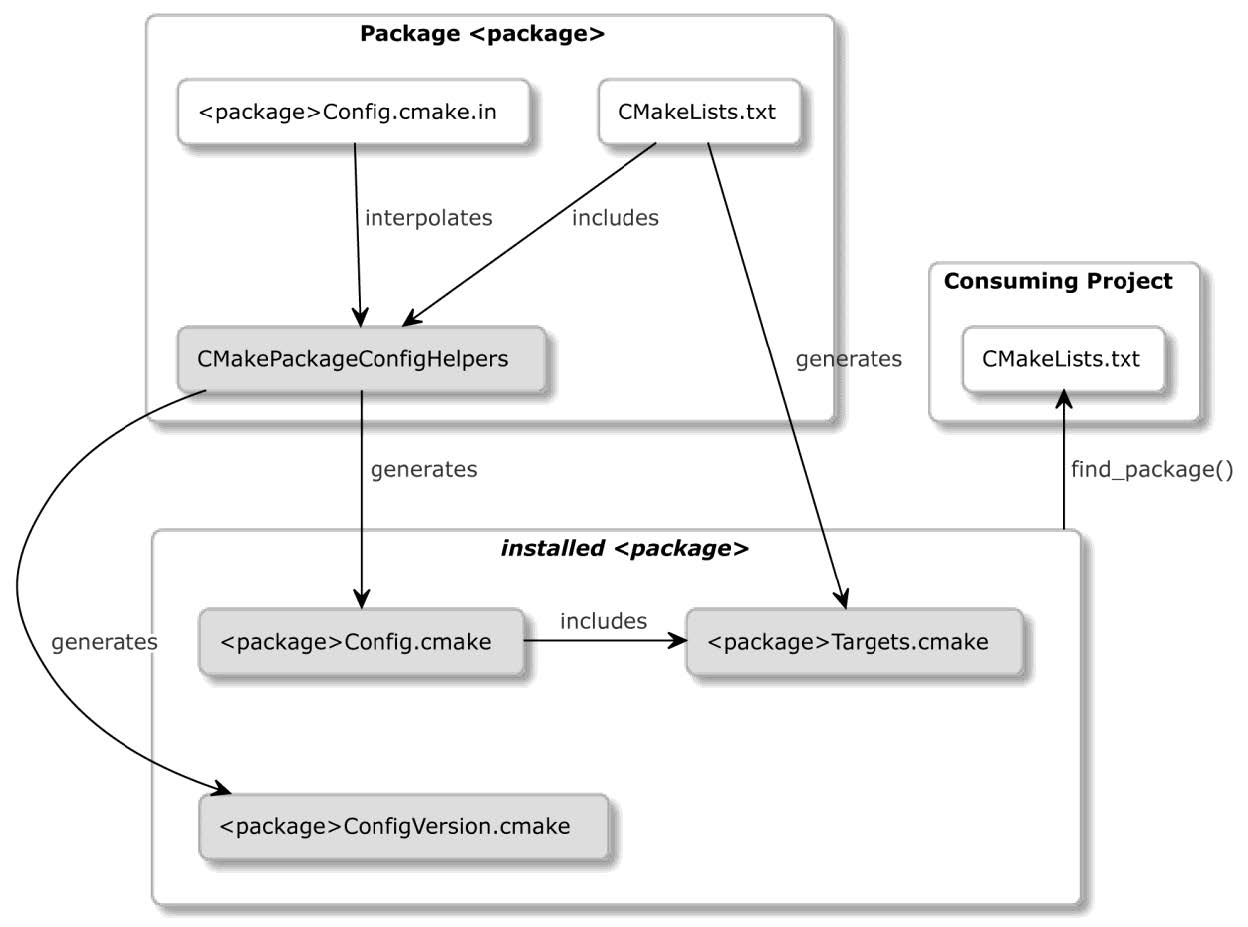
\includegraphics[width=0.8\textwidth]{content/3/chapter11/images/1.jpg}\\
图11.1 高级包的文件结构
\end{center}

包的所有必需的子依赖项也必须在包配置文件中找到。这可以通过调用CMakeFindDependencyMacro助手模块中的find\_dependency()宏来实现。我们在第7章中学习了如何使用。

若决定向其他项目公开宏或函数,建议将定义放在一个单独的文件中,这样就可以使用include()包含配置文件了。

有趣的是,CMakePackageConfigHelpers还提供了辅助指令来生成包的版本文件。

\subsubsubsection{11.4.5\hspace{0.2cm}生成包版本文件}

随着包的增长,将慢慢获得新的功能,旧的功能将会标记为弃用,并最终删除。在使用包的开发人员可用的变更日志中跟踪这些修改是很重要的。当需要一个特定的特性时,开发人员可以找到支持它的最低版本,并使用它作为find\_package()的参数:

\begin{lstlisting}[style=styleCMake]
find_package(Calc 1.2.3 REQUIRED)
\end{lstlisting}

CMake将在配置文件中搜索Calc,并检查是否有一个名为<config-file>-version.cmake的版本文件,或存在于同一目录中的<config-file>Version.cmake,即CalcConfigVersion.cmake。接下来,将读取该文件的版本信息以及它提供的与其他版本的兼容性。若没有按要求安装1.2.3版本,但可能安装了1.3.5,将标记为与任何旧版本“兼容”。CMake很乐意接受这样的包,因为它知道包供应商提供向了后兼容。

可以使用CMakePackageConfigHelpers实用模块通过write\_basic\_package\_version\_file()来生成包的版本文件:

\begin{lstlisting}[style=styleCMake]
write_basic_package_version_file(<filename> [VERSION <ver>]
	COMPATIBILITY <AnyNewerVersion | SameMajorVersion |
				   SameMinorVersion | ExactVersion>
	[ARCH_INDEPENDENT]
)
\end{lstlisting}

首先,需要提供想要创建的工件的<filename>属性,必须遵循前面概述的规则。除此之外,应该在构建树中存储所有生成的文件。

可选地,可以传递一个显式的VERSION(通常的格式,major.minor.patch)。若不这样做,则将使用project()中提供的版本。

COMPATIBILITY关键字的含义不言自明:

\begin{itemize}
\item 
ExactVersion必须匹配版本的所有三个组件,不支持范围版本: find\_package(<package> 1.2.8...1.3.4).

\item 
若前两个组件相同(忽略patch),则SameMinorVersion匹配。

\item 
若第一个组件相同(忽略minor和patch),则匹配SameMajorVersion。

\item 
AnyNewerVersion似乎有一个相反的名称:将匹配任何旧版本。换句话说,版本1.4.2上的将很适合find\_package(<package> 1.2.8).
\end{itemize}

通常,包都必须为与使用项目相匹配的相同架构构建(执行精确检查)。但对于不编译的包(只编译头库、宏包等),可以指定ARCH\_INDEPENDENT关键字来跳过此检查。

现在,举一个实际的例子。下面的代码展示了如何为06-install-export示例中启动的项目提供版本文件:

\begin{lstlisting}[style=styleCMake]
# chapter-11/10-version-file/CMakeLists.txt (fragment)

cmake_minimum_required(VERSION 3.20.0)
project(VersionFile VERSION 1.2.3 LANGUAGES CXX)
...
include(CMakePackageConfigHelpers)
write_basic_package_version_file(
	"${CMAKE_CURRENT_BINARY_DIR}/CalcConfigVersion.cmake"
	COMPATIBILITY AnyNewerVersion
)
install(FILES "CalcConfig.cmake"
	"${CMAKE_CURRENT_BINARY_DIR}/CalcConfigVersion.cmake"
	DESTINATION ${CMAKE_INSTALL_LIBDIR}/calc/cmake
)
\end{lstlisting}

方便起见,需要在文件顶部的project()中配置包的版本。需要通过添加LANGUAGE关键字,从简短的project(<name> <languages>)语法切换到显式的完整语法。

包含辅助程序模块之后,调用生成命令将文件写入构建树,其名称符合find\_package()要求的模式。这里,故意跳过VERSION关键字,以便从PROJECT\_VERSION变量中读取版本。我们还将我们的包标记为完全向后兼容COMPATIBILITY AnyNewerVersion。之后,将包版本文件安装到与CalcConfig.cmake相同的目录。就是这样,包已经完全配置好了。

下一节中,将学习什么是组件,以及如何将它们与包一起使用。







